\subsection{Открытые и замкнутые множества в пространстве и подпространстве}
    
    \begin{theorem-non}
        $(X, d)$ -метр пространство $Y \subset X$. Тогда:
        \begin{enumerate}
            \item $A \subset Y$ открыто в $Y \Longleftrightarrow$ найдется открытое множество $G \subset X$, т.ч. $A=G\cap Y$ \vspace*{0,5cm} \\
            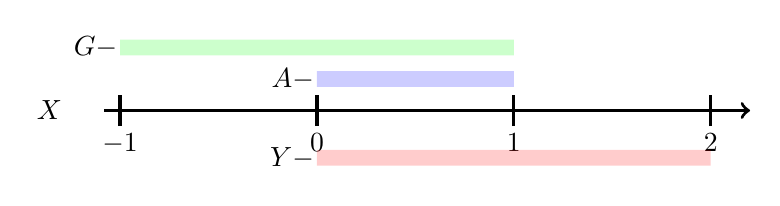
\begin{tikzpicture}[mydrawstyle/.style={draw=black, very thick}, x=1mm, y=1mm, z=1mm]
                \draw[mydrawstyle, ->](-2,30)--(80,30);
                \draw[mydrawstyle] node at (-6,30)[left]{$X$};
                \draw[mydrawstyle] node at (26,24)[left]{$Y - $};
                \draw[mydrawstyle] node at (1,38)[left]{$G - $};
                \draw[mydrawstyle] node at (26,34)[left]{$A - $};
                \draw[mydrawstyle](0,28)--(0,32) node[below=10]{$-1$};
                \draw[mydrawstyle](25,28)--(25,32) node[below=10]{$0$};
                \draw[mydrawstyle](50,28)--(50,32) node[below=10]{$1$};
                \draw[mydrawstyle](75,28)--(75,32) node[below=10]{$2$};
                \fill[fill=blue, opacity=0.2](25,33)--(25,35)--(50,35)--(50,33)--(25,33);
                \fill[fill=red, opacity=0.2](25,23)--(25,25)--(75,25)--(75,23)--(25,23);
                \fill[fill=green, opacity=0.2](0,37)--(0,39)--(50,39)--(50,37)--(0,37);
              \end{tikzpicture}
            \begin{proof}
                $a \in A \Longrightarrow \exists r_a>0 : B_{r_a}^Y(a)$ (т.е. шары в $Y$) $\subset A$. Далее
                \begin{center}
                    $G:= \underset{a\in A}{\cup} B_{r_a}^X(a) = \underset{a\in A}{\cup} \{x \in X: d(x, a)<r_a\} \Longrightarrow$
                \end{center}
                $G$ - открытое (объединение любого числа открытых - открытое)
                Доказать: $G\cap Y = A$
                $G \supset A, Y \supset A \Longrightarrow G\cap Y \supset A$. Докажем обратное включение.
                \begin{center}
                    $B_{r_a}^X(a)\cap Y = B_{r_a}^Y \subset A$ \vspace*{0,2cm} \\
                    $G\cap Y = \underset{a\in A}{\cup}(B_{r_a}^X(a) \cap Y) \subset A \Longrightarrow G\cap Y \subset A$
                \end{center}
                Доказали "$\Longrightarrow$". Теперь докажем "$\Longleftarrow$"\\
                $G$ - открыто в $Y$. Доказать, что $A := G\cap Y$ - открыто в $Y$
                $a \in A \Longrightarrow a \in G$, $G$ - открыто$ \Longrightarrow \exists r>0 : B_r^X(a) \subset G \Longrightarrow B_r^X(a)\cap Y = B_r^Y(a) \subset G\cap Y$, то есть $A$ открыто в $Y$.
            \end{proof}
            \item $A \subset Y$ замкнутое в $Y \Longleftrightarrow$ найдется замкнутое множество $F \in X $, т. ч $A = F\cap Y$
            \begin{proof}
                $A$ - замкнуто в $Y \Longleftrightarrow Y\setminus A$ - открыто в $Y \Longleftrightarrow \\
                \exists$ открытое $G \in X : Y\setminus A = G\cap Y \Longleftrightarrow \\
                F := X\setminus G$ - замкнутое в $X$, при этом $A = Y\setminus (G\cap Y) = Y\cap (X\setminus G)$ \vspace*{0,2cm}\\
                \framebox[1.02\width]{С первого взгляда неочевидный переход, но следует из вложенности $Y$ и $G$ в $X = Y\cap F$.} \par
            \end{proof}
        \end{enumerate}
    \end{theorem-non}